
%% bare_jrnl_comsoc.tex
%% V1.4b
%% 2015/08/26
%% by Michael Shell
%% see http://www.michaelshell.org/
%% for current contact information.
%%
%% This is a skeleton file demonstrating the use of IEEEtran.cls
%% (requires IEEEtran.cls version 1.8b or later) with an IEEE
%% Communications Society journal paper.
%%
%% Support sites:
%% http://www.michaelshell.org/tex/ieeetran/
%% http://www.ctan.org/pkg/ieeetran
%% and
%% http://www.ieee.org/

%%*************************************************************************
%% Legal Notice:
%% This code is offered as-is without any warranty either expressed or
%% implied; without even the implied warranty of MERCHANTABILITY or
%% FITNESS FOR A PARTICULAR PURPOSE! 
%% User assumes all risk.
%% In no event shall the IEEE or any contributor to this code be liable for
%% any damages or losses, including, but not limited to, incidental,
%% consequential, or any other damages, resulting from the use or misuse
%% of any information contained here.
%%
%% All comments are the opinions of their respective authors and are not
%% necessarily endorsed by the IEEE.
%%
%% This work is distributed under the LaTeX Project Public License (LPPL)
%% ( http://www.latex-project.org/ ) version 1.3, and may be freely used,
%% distributed and modified. A copy of the LPPL, version 1.3, is included
%% in the base LaTeX documentation of all distributions of LaTeX released
%% 2003/12/01 or later.
%% Retain all contribution notices and credits.
%% ** Modified files should be clearly indicated as such, including  **
%% ** renaming them and changing author support contact information. **
%%*************************************************************************


% *** Authors should verify (and, if needed, correct) their LaTeX system  ***
% *** with the testflow diagnostic prior to trusting their LaTeX platform ***
% *** with production work. The IEEE's font choices and paper sizes can   ***
% *** trigger bugs that do not appear when using other class files.       ***                          ***
% The testflow support page is at:
% http://www.michaelshell.org/tex/testflow/



\documentclass[journal,comsoc]{IEEEtran}
%
% If IEEEtran.cls has not been installed into the LaTeX system files,
% manually specify the path to it like:
% \documentclass[journal,comsoc]{../sty/IEEEtran}


\usepackage[T1]{fontenc}% optional T1 font encoding


% Some very useful LaTeX packages include:
% (uncomment the ones you want to load)


% *** MISC UTILITY PACKAGES ***
%
%\usepackage{ifpdf}
% Heiko Oberdiek's ifpdf.sty is very useful if you need conditional
% compilation based on whether the output is pdf or dvi.
% usage:
% \ifpdf
%   % pdf code
% \else
%   % dvi code
% \fi
% The latest version of ifpdf.sty can be obtained from:
% http://www.ctan.org/pkg/ifpdf
% Also, note that IEEEtran.cls V1.7 and later provides a builtin
% \ifCLASSINFOpdf conditional that works the same way.
% When switching from latex to pdflatex and vice-versa, the compiler may
% have to be run twice to clear warning/error messages.






% *** CITATION PACKAGES ***
%
\usepackage{cite}
% cite.sty was written by Donald Arseneau
% V1.6 and later of IEEEtran pre-defines the format of the cite.sty package
% \cite{} output to follow that of the IEEE. Loading the cite package will
% result in citation numbers being automatically sorted and properly
% "compressed/ranged". e.g., [1], [9], [2], [7], [5], [6] without using
% cite.sty will become [1], [2], [5]--[7], [9] using cite.sty. cite.sty's
% \cite will automatically add leading space, if needed. Use cite.sty's
% noadjust option (cite.sty V3.8 and later) if you want to turn this off
% such as if a citation ever needs to be enclosed in parenthesis.
% cite.sty is already installed on most LaTeX systems. Be sure and use
% version 5.0 (2009-03-20) and later if using hyperref.sty.
% The latest version can be obtained at:
% http://www.ctan.org/pkg/cite
% The documentation is contained in the cite.sty file itself.






% *** GRAPHICS RELATED PACKAGES ***
%
%\usepackage[caption=false,font=footnotesize]{subfig}
\usepackage{graphicx}
\usepackage{caption}
%\graphicspath{{../figuras/}}
\ifCLASSINFOpdf
   %\usepackage[pdftex]{graphicx}
  % declare the path(s) where your graphic files are
  %\graphicspath{{../figuras/}}
  % and their extensions so you won't have to specify these with
  % every instance of \includegraphics
  % \DeclareGraphicsExtensions{.pdf,.jpeg,.png}
\else
  % or other class option (dvipsone, dvipdf, if not using dvips). graphicx
  % will default to the driver specified in the system graphics.cfg if no
  % driver is specified.
  % \usepackage[dvips]{graphicx}
  % declare the path(s) where your graphic files are
  % \graphicspath{{../eps/}}
  % and their extensions so you won't have to specify these with
  % every instance of \includegraphics
  % \DeclareGraphicsExtensions{.eps}
\fi
% graphicx was written by David Carlisle and Sebastian Rahtz. It is
% required if you want graphics, photos, etc. graphicx.sty is already
% installed on most LaTeX systems. The latest version and documentation
% can be obtained at: 
% http://www.ctan.org/pkg/graphicx
% Another good source of documentation is "Using Imported Graphics in
% LaTeX2e" by Keith Reckdahl which can be found at:
% http://www.ctan.org/pkg/epslatex
%
% latex, and pdflatex in dvi mode, support graphics in encapsulated
% postscript (.eps) format. pdflatex in pdf mode supports graphics
% in .pdf, .jpeg, .png and .mps (metapost) formats. Users should ensure
% that all non-photo figures use a vector format (.eps, .pdf, .mps) and
% not a bitmapped formats (.jpeg, .png). The IEEE frowns on bitmapped formats
% which can result in "jaggedy"/blurry rendering of lines and letters as
% well as large increases in file sizes.
%
% You can find documentation about the pdfTeX application at:
% http://www.tug.org/applications/pdftex





% *** MATH PACKAGES ***
%
\usepackage{amsmath}
% A popular package from the American Mathematical Society that provides
% many useful and powerful commands for dealing with mathematics.
% Do NOT use the amsbsy package under comsoc mode as that feature is
% already built into the Times Math font (newtxmath, mathtime, etc.).
% 
% Also, note that the amsmath package sets \interdisplaylinepenalty to 10000
% thus preventing page breaks from occurring within multiline equations. Use:
\interdisplaylinepenalty=2500
% after loading amsmath to restore such page breaks as IEEEtran.cls normally
% does. amsmath.sty is already installed on most LaTeX systems. The latest
% version and documentation can be obtained at:
% http://www.ctan.org/pkg/amsmath


% Select a Times math font under comsoc mode or else one will automatically
% be selected for you at the document start. This is required as Communications
% Society journals use a Times, not Computer Modern, math font.
\usepackage[cmintegrals]{newtxmath}
% The freely available newtxmath package was written by Michael Sharpe and
% provides a feature rich Times math font. The cmintegrals option, which is
% the default under IEEEtran, is needed to get the correct style integral
% symbols used in Communications Society journals. Version 1.451, July 28,
% 2015 or later is recommended. Also, do *not* load the newtxtext.sty package
% as doing so would alter the main text font.
% http://www.ctan.org/pkg/newtx
%
% Alternatively, you can use the MathTime commercial fonts if you have them
% installed on your system:
%\usepackage{mtpro2}
%\usepackage{mt11p}
%\usepackage{mathtime}


%\usepackage{bm}
% The bm.sty package was written by David Carlisle and Frank Mittelbach.
% This package provides a \bm{} to produce bold math symbols.
% http://www.ctan.org/pkg/bm





% *** SPECIALIZED LIST PACKAGES ***
%
%\usepackage{algorithmic}
% algorithmic.sty was written by Peter Williams and Rogerio Brito.
% This package provides an algorithmic environment fo describing algorithms.
% You can use the algorithmic environment in-text or within a figure
% environment to provide for a floating algorithm. Do NOT use the algorithm
% floating environment provided by algorithm.sty (by the same authors) or
% algorithm2e.sty (by Christophe Fiorio) as the IEEE does not use dedicated
% algorithm float types and packages that provide these will not provide
% correct IEEE style captions. The latest version and documentation of
% algorithmic.sty can be obtained at:
% http://www.ctan.org/pkg/algorithms
% Also of interest may be the (relatively newer and more customizable)
% algorithmicx.sty package by Szasz Janos:
% http://www.ctan.org/pkg/algorithmicx




% *** ALIGNMENT PACKAGES ***
%
%\usepackage{array}
% Frank Mittelbach's and David Carlisle's array.sty patches and improves
% the standard LaTeX2e array and tabular environments to provide better
% appearance and additional user controls. As the default LaTeX2e table
% generation code is lacking to the point of almost being broken with
% respect to the quality of the end results, all users are strongly
% advised to use an enhanced (at the very least that provided by array.sty)
% set of table tools. array.sty is already installed on most systems. The
% latest version and documentation can be obtained at:
% http://www.ctan.org/pkg/array


% IEEEtran contains the IEEEeqnarray family of commands that can be used to
% generate multiline equations as well as matrices, tables, etc., of high
% quality.




% *** SUBFIGURE PACKAGES ***
%\ifCLASSOPTIONcompsoc
%  \usepackage[caption=false,font=normalsize,labelfont=sf,textfont=sf]{subfig}
%\else
%  \usepackage[caption=false,font=footnotesize]{subfig}
%\fi
% subfig.sty, written by Steven Douglas Cochran, is the modern replacement
% for subfigure.sty, the latter of which is no longer maintained and is
% incompatible with some LaTeX packages including fixltx2e. However,
% subfig.sty requires and automatically loads Axel Sommerfeldt's caption.sty
% which will override IEEEtran.cls' handling of captions and this will result
% in non-IEEE style figure/table captions. To prevent this problem, be sure
% and invoke subfig.sty's "caption=false" package option (available since
% subfig.sty version 1.3, 2005/06/28) as this is will preserve IEEEtran.cls
% handling of captions.
% Note that the Computer Society format requires a larger sans serif font
% than the serif footnote size font used in traditional IEEE formatting
% and thus the need to invoke different subfig.sty package options depending
% on whether compsoc mode has been enabled.
%
% The latest version and documentation of subfig.sty can be obtained at:
% http://www.ctan.org/pkg/subfig




% *** FLOAT PACKAGES ***
%
%\usepackage{fixltx2e}
% fixltx2e, the successor to the earlier fix2col.sty, was written by
% Frank Mittelbach and David Carlisle. This package corrects a few problems
% in the LaTeX2e kernel, the most notable of which is that in current
% LaTeX2e releases, the ordering of single and double column floats is not
% guaranteed to be preserved. Thus, an unpatched LaTeX2e can allow a
% single column figure to be placed prior to an earlier double column
% figure.
% Be aware that LaTeX2e kernels dated 2015 and later have fixltx2e.sty's
% corrections already built into the system in which case a warning will
% be issued if an attempt is made to load fixltx2e.sty as it is no longer
% needed.
% The latest version and documentation can be found at:
% http://www.ctan.org/pkg/fixltx2e

%\usepackage{fixltx2e}
%\usepackage{stfloats}
% stfloats.sty was written by Sigitas Tolusis. This package gives LaTeX2e
% the ability to do double column floats at the bottom of the page as well
% as the top. (e.g., "\begin{figure*}[!b]" is not normally possible in
% LaTeX2e). It also provides a command:
%\fnbelowfloat
% to enable the placement of footnotes below bottom floats (the standard
% LaTeX2e kernel puts them above bottom floats). This is an invasive package
% which rewrites many portions of the LaTeX2e float routines. It may not work
% with other packages that modify the LaTeX2e float routines. The latest
% version and documentation can be obtained at:
% http://www.ctan.org/pkg/stfloats
% Do not use the stfloats baselinefloat ability as the IEEE does not allow
% \baselineskip to stretch. Authors submitting work to the IEEE should note
% that the IEEE rarely uses double column equations and that authors should try
% to avoid such use. Do not be tempted to use the cuted.sty or midfloat.sty
% packages (also by Sigitas Tolusis) as the IEEE does not format its papers in
% such ways.
% Do not attempt to use stfloats with fixltx2e as they are incompatible.
% Instead, use Morten Hogholm'a dblfloatfix which combines the features
% of both fixltx2e and stfloats:
%
% \usepackage{dblfloatfix}
% The latest version can be found at:
% http://www.ctan.org/pkg/dblfloatfix




%\ifCLASSOPTIONcaptionsoff
%  \usepackage[nomarkers]{endfloat}
% \let\MYoriglatexcaption\caption
% \renewcommand{\caption}[2][\relax]{\MYoriglatexcaption[#2]{#2}}
%\fi
% endfloat.sty was written by James Darrell McCauley, Jeff Goldberg and 
% Axel Sommerfeldt. This package may be useful when used in conjunction with 
% IEEEtran.cls'  captionsoff option. Some IEEE journals/societies require that
% submissions have lists of figures/tables at the end of the paper and that
% figures/tables without any captions are placed on a page by themselves at
% the end of the document. If needed, the draftcls IEEEtran class option or
% \CLASSINPUTbaselinestretch interface can be used to increase the line
% spacing as well. Be sure and use the nomarkers option of endfloat to
% prevent endfloat from "marking" where the figures would have been placed
% in the text. The two hack lines of code above are a slight modification of
% that suggested by in the endfloat docs (section 8.4.1) to ensure that
% the full captions always appear in the list of figures/tables - even if
% the user used the short optional argument of \caption[]{}.
% IEEE papers do not typically make use of \caption[]'s optional argument,
% so this should not be an issue. A similar trick can be used to disable
% captions of packages such as subfig.sty that lack options to turn off
% the subcaptions:
% For subfig.sty:
% \let\MYorigsubfloat\subfloat
% \renewcommand{\subfloat}[2][\relax]{\MYorigsubfloat[]{#2}}
% However, the above trick will not work if both optional arguments of
% the \subfloat command are used. Furthermore, there needs to be a
% description of each subfigure *somewhere* and endfloat does not add
% subfigure captions to its list of figures. Thus, the best approach is to
% avoid the use of subfigure captions (many IEEE journals avoid them anyway)
% and instead reference/explain all the subfigures within the main caption.
% The latest version of endfloat.sty and its documentation can obtained at:
% http://www.ctan.org/pkg/endfloat
%
% The IEEEtran \ifCLASSOPTIONcaptionsoff conditional can also be used
% later in the document, say, to conditionally put the References on a 
% page by themselves.




% *** PDF, URL AND HYPERLINK PACKAGES ***
%
%\usepackage{url}
% url.sty was written by Donald Arseneau. It provides better support for
% handling and breaking URLs. url.sty is already installed on most LaTeX
% systems. The latest version and documentation can be obtained at:
% http://www.ctan.org/pkg/url
% Basically, \url{my_url_here}.




% *** Do not adjust lengths that control margins, column widths, etc. ***
% *** Do not use packages that alter fonts (such as pslatex).         ***
% There should be no need to do such things with IEEEtran.cls V1.6 and later.
% (Unless specifically asked to do so by the journal or conference you plan
% to submit to, of course. )


% correct bad hyphenation here
\hyphenation{op-tical net-works semi-conduc-tor}


\begin{document}
%
% paper title
% Titles are generally capitalized except for words such as a, an, and, as,
% at, but, by, for, in, nor, of, on, or, the, to and up, which are usually
% not capitalized unless they are the first or last word of the title.
% Linebreaks \\ can be used within to get better formatting as desired.
% Do not put math or special symbols in the title.
\title{Implementación de un Transmisor de ISDB-T Abierto Bajo el Paradigma de Radio Definida por Software}
%
%
% author names and IEEE memberships
% note positions of commas and nonbreaking spaces ( ~ ) LaTeX will not break
% a structure at a ~ so this keeps an author's name from being broken across
% two lines.
% use \thanks{} to gain access to the first footnote area
% a separate \thanks must be used for each paragraph as LaTeX2e's \thanks
% was not built to handle multiple paragraphs
%

\author{Javier~Hernández~(javier.hernandez@fing.edu.uy),
        Santiago~Castro~(santiago.castro@fing.edu.uy)}% <-this % stops a space
% <-this % stops a space
%\thanks{}% <-this % stops a space
%\thanks{}}

% note the % following the last \IEEEmembership and also \thanks - 
% these prevent an unwanted space from occurring between the last author name
% and the end of the author line. i.e., if you had this:
% 
% \author{....lastname \thanks{...} \thanks{...} }
%                     ^------------^------------^----Do not want these spaces!
%
% a space would be appended to the last name and could cause every name on that
% line to be shifted left slightly. This is one of those "LaTeX things". For
% instance, "\textbf{A} \textbf{B}" will typeset as "A B" not "AB". To get
% "AB" then you have to do: "\textbf{A}\textbf{B}"
% \thanks is no different in this regard, so shield the last } of each \thanks
% that ends a line with a % and do not let a space in before the next \thanks.
% Spaces after \IEEEmembership other than the last one are OK (and needed) as
% you are supposed to have spaces between the names. For what it is worth,
% this is a minor point as most people would not even notice if the said evil
% space somehow managed to creep in.



% The paper headers
%\markboth{}%
%{}
% The only time the second header will appear is for the odd numbered pages
% after the title page when using the twoside option.
% 
% *** Note that you probably will NOT want to include the author's ***
% *** name in the headers of peer review papers.                   ***
% You can use \ifCLASSOPTIONpeerreview for conditional compilation here if
% you desire.




% If you want to put a publisher's ID mark on the page you can do it like
% this:
%\IEEEpubid{0000--0000/00\$00.00~\copyright~2015 IEEE}
% Remember, if you use this you must call \IEEEpubidadjcol in the second
% column for its text to clear the IEEEpubid mark.



% use for special paper notices
%\IEEEspecialpapernotice{(Invited Paper)}




% make the title area
\maketitle

% As a general rule, do not put math, special symbols or citations
% in the abstract or keywords.
\begin{abstract}
ISDB-T es el principal estándar adoptado en América Latina para la difusión de televisión digital terrestre. Hoy en día el estándar está consolidado en la región, los países de América Latina han realizado importantes inversiones para desplegar el nuevo sistema de televisión digital terrestre basado en este estándar. Esto nos lleva a investigar y desarrollar nuevas posibilidades en lo que respecta al sistema de televisión digital. En este artículo presentamos gr-isdbt-tx, un transmisor ISDB-T abierto, libre y gratuito totalmente basado en software, implementado en GNU Radio. Esta implementación es capaz de generar una señal de televisión digital compatible con cualquier televisor digital homologado para ISDB-T. También permite que estudiantes, profesionales e investigadores puedan conocer al detalle cómo es que funciona un transmisor de televisión digital, sin necesidad de costear equipos de gran valor económico.
En conjunción con “gr-isdbt: Un receptor ISDB-T fullseg abierto y libre implementado en GNU Radio”, el usuario tiene una poderosa herramienta para correr un sistema de televisión digital de punta a punta, y así explorar y probar el comportamiento de un sistema de comunicación complejo sin ningún tipo de hardware.
En este artículo presentamos el transmisor desarrollado, así como sus fundamentos y los problemas más relevantes que han tenido que ser resueltos para lograr una implementación exitosa. También presentamos algunas pruebas y sus resultados. 

\end{abstract}

% Note that keywords are not normally used for peerreview papers.
\begin{IEEEkeywords}
Integrated Services Digital Broadcasting, GNU Radio, Software Defined Radio.
\end{IEEEkeywords}






% For peer review papers, you can put extra information on the cover
% page as needed:
% \ifCLASSOPTIONpeerreview
% \begin{center} \bfseries EDICS Category: 3-BBND \end{center}
% \fi
%
% For peerreview papers, this IEEEtran command inserts a page break and
% creates the second title. It will be ignored for other modes.
\IEEEpeerreviewmaketitle



\section{Introducción}
% The very first letter is a 2 line initial drop letter followed
% by the rest of the first word in caps.
% 
% form to use if the first word consists of a single letter:
% \IEEEPARstart{A}{demo} file is ....
% 
% form to use if you need the single drop letter followed by
% normal text (unknown if ever used by the IEEE):
% \IEEEPARstart{A}{}demo file is ....
% 
% Some journals put the first two words in caps:
% \IEEEPARstart{T}{his demo} file is ....
% 
% Here we have the typical use of a "T" for an initial drop letter
% and "HIS" in caps to complete the first word.
Los antiguos sistemas de televisión analógica están siendo reemplazados por los nuevos sistemas digitales. Existe una innumerable cantidad de mejoras y ventajas respecto a los antiguos, como por ejemplo una mayor eficiencia espectral, mejor calidad de audio y video, la posibilidad de transmitir múltiples programas al mismo tiempo en el mismo canal, y la utilización de canales de datos. El enorme crecimiento que han tenido las comunicaciones inalámbricas en los últimos tiempos, ha hecho que el espectro radioeléctrico se convierta en un recurso natural finito extremadamente valioso. Varios países ya han transitado el camino “apagón analógico”, reemplazando definitivamente los sistemas de televisión analógica. Sin embargo hay muchos otros en los que aún conviven ambos sistemas de teledifusión.
El despliegue de un nuevo sistema de televisión digital es una tarea mayúscula, tal como en otros campos de las comunicaciones inalámbricas surgen distintas soluciones para el mismo problema. Respecto a los sistemas de televisión digital, se pueden encontrar los siguientes estándares: ISDB (Integrated Services Digital Broadcasting) es el estándar japonés, DVB (Digital Video Broadcasting) es el estándar europeo, ATSC (Advanced Television Systems Committee) es el estándar norteamericano y DTMB (Digital Terrestrial Multimedia Broadcast) es el estándar chino.

Este trabajo se enfoca en el estándar ISDB-T el cual ha sido ampliamente adoptado por los países de América Latina. Muchos países aún se encuentran desplegando sus sistemas de televisión digital, para lograr un despliegue exitoso es imprescindible contar con una comprensión profunda de la norma. Este grado de dominio no sería posible alcanzarlo si no se conoce en detalle todo el sistema, desde la etapa de transmisión hasta la etapa de recepción. Las compañías que fabrican esta clase de equipamiento son algunas pocas en el mundo y sus soluciones no suelen estar al alcance de todos. 

Las Radios Definidas por Software (SDR por sus siglas en inglés) son una gran alternativa para desarrollar sistemas de comunicación. Se trata de un nuevo paradigma donde los sistemas de radiocomunicaciones, tradicionalmente implementados en hardware, son en cambio implementados por software. Esto típicamente se lleva a cabo a través de una computadora personal encargada de ejecutar el software, y un hardware genérico que se encarga de sintonizar, filtrar y muestrear la señal de radio a cierta tasa. De esta manera la señal puede ser procesada por la computadora. Hay una gran variedad de estos equipos que van desde unos pocos dólares hasta algunos cientos o incluso miles de dólares. El paradigma de la radio definida por software permite lograr una implementación completa de sistemas de radiocomunicaciones de manera económica y sencilla en cierto sentido. 

En este trabajo en particular, utilizamos una PC de propósito general junto con equipos basados en SDR como lo son el USRP B100 (Universal Software Radio Peripheral de Ettus)\cite{b100} o el HackRF One (de Great Scott Gadgets) \cite{GreatScottGadgets} que cumplen con la tasa de muestreo requerida por el estándar ISDB-T.
Para el desarrollo utilizamos el toolkit de GNU Radio, se trata de un software ampliamente utilizado para el desarrollo de radios definidas por software. Provee de bloques de procesamiento de señal de propósito general como filtros, re-samplers, moduladores y demoduladores analógicos y digitales. Estos bloques pueden ser combinados para lograr diferentes sistemas de comunicación. También es posible la implementación de nuevos bloques personalizados por parte de los usuarios, de manera de contribuir con el código fuente de GNU Radio. Esto hace que la comunidad de GNU Radio sea muy activa y resulte en una contribución continua de los usuarios tanto en el desarrollo de nuevas radios definidas por software o el testeo de otras implementaciones.

En este trabajo presentamos gr-isdbt-tx (https://github.com/jhernandezbaraibar/gr-isdbt-Tx), un transmisor de ISDB-T abierto bajo el paradigma de radio definida por software, que continúa y complementa la línea de trabajo comenzada con el receptor gr-isdbt. 

Este transmisor ha sido implementado completamente en GNU Radio y puede tomar hasta tres flujos de entrada MPEG-2 tal como lo establece el estándar. Tiene la posibilidad de trabajar tanto en modo one-seg como en full-seg, y el usuario cuenta con la libertad de establecer los parámetros de configuración del sistema. El desarrollo sobre GNU Radio hace que, con solamente un PC, el usuario pueda correr un sistema de televisión digital de punta a punta integrando gr-isdbt-tx con gr-isdbt. Alternativamente con un hardware SDR, como el USRP B100, es posible transmitir la señal por el aire hacia cualquier televisor de uso doméstico compatible con ISDB-T.

En lo que sigue se presenta una descripción del estándar ISDB-T
---------------------------
Los detalles de programación y los algoritmos utilizados pueden ser consultados en detalle en el repositorio del proyecto. Aqui describiremos el funcionamiento del sistema
\begin{figure*}[!h]
\centering
%\captionsetup{justification=centering}
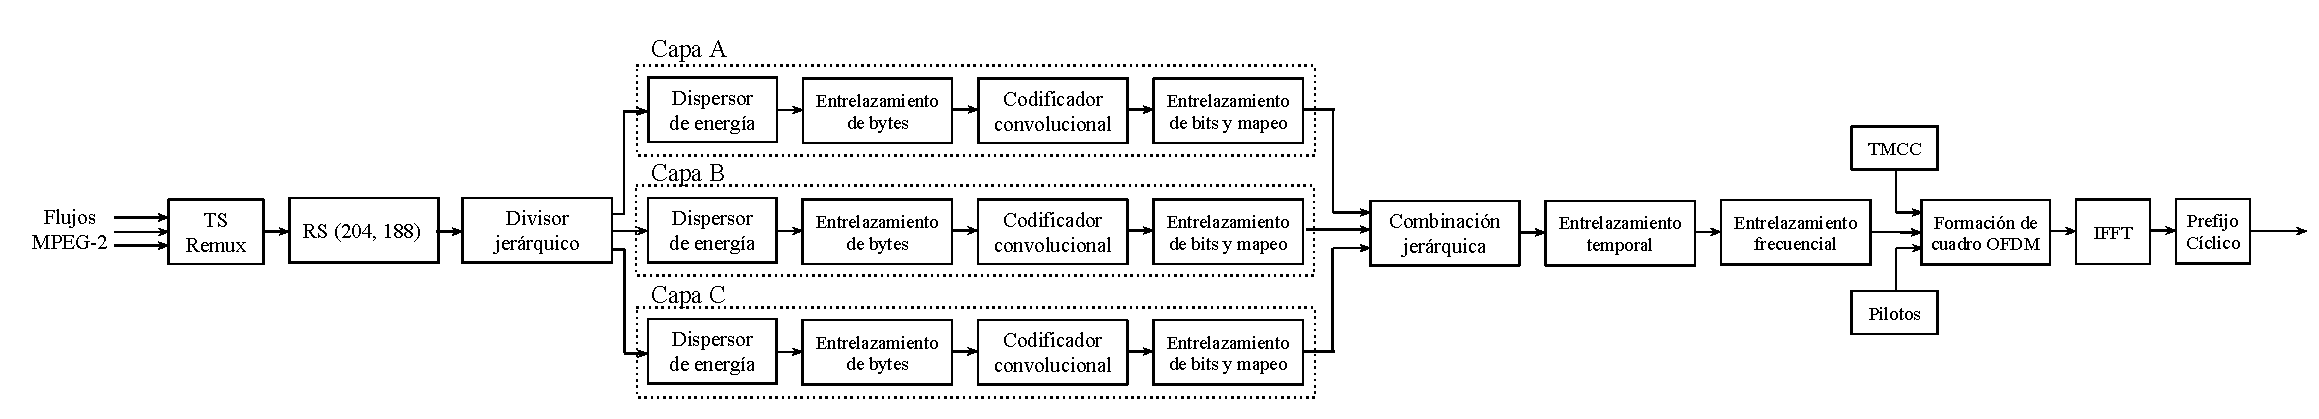
\includegraphics[width=7.1in]{figuras/esquema-tx}
% where an .eps filename suffix will be assumed under latex, 
% and a .pdf suffix will be assumed for pdflatex; or what has been declared
% via \DeclareGraphicsExtensions.
\caption{Esquema del sistema transmisor ISDB-T.}
\label{esquema-tx}
\end{figure*}

\section{El estándar ISDB-T}
El estándar de television digital terrestre ISDB-T puede ser caracterizado en cuatro grandes etapas: la conformación del Broadcast Transport Stream (BTS), la codificación de canal, la formación del cuadro OFDM, y la puesta en el aire de la señal. En la figura \ref{esquema_isdbt} se presenta el esquema completo del sistema transmisor.
El sistema admite como fuente de datos hasta tres flujos de transporte MPEG-2 \cite{MPEG}. Cada flujo está conformado por una secuencia de paquetes denominados \textit{Transport Stream Packet} (TSP) de 188 bytes. Los flujos MPEG-2 son multiplexados por el bloque TS Remux en un único flujo llamado \textit{Broadcast Transport Stream} (BTS); además de la multiplexación de los TSP el TS Remux tiene otras tareas como el agregado de cierta información jerárquica en los paquetes.

Una de las características destacables de ISDB-T es la posibilidad de la transmisión jerárquica de la información, esto es, que cada flujo MPEG-2 puede ser transmitido con una configuración propia con distintos grados de robustez. A la transmisión de un flujo MPEG-2 con su configuración jerárquica se lo denomina \textit{capa jerárquica} y el estándar permite transmitir hasta tres capas en simultáneo. Cada capa tiene asignada un conjunto de portadoras en el espectro que más adelante se analizará su conformación.

Una vez conformado el BTS se comienza a robustecer la señal agregando redundancia y utilizando distintos tipos de entrelazamientos. En los sistemas de comunicaciones es común encontrar que se utilicen códigos correctores de errrores concatenados, esto aumenta significativamente el desempeño de los mismos. En ISDB-T se utiliza como código exterior un Reed-Solomon (204,188) y un código convolucional (FEC) como código interior.  

Como cada flujo debe ser procesado por separado es necesario que a cada uno se le aplique un proceso según la configuración jerárquica elegida. Es por esto que hay un bloque \textbf{divisor jerárquico} encargado de separar el BTS en tres flujos y encaminarlos según lo que corresponda.

El robustecimiento de la señal se realiza con distintos objetivos, por ejemplo para evitar el fading en frecuencia, las ráfagas de errores, ...., etc. El bloque dispersor de energía tiene como objetivo eliminar posibles largas secuencias de unos o ceros que puedan haber en el flujo de transporte. De otra manera podrían haber errores de sincronismo y también habrían porciones del espectro donde se concentraría la energía, quedando así subutilizado este recurso. El dispersor de energía utiliza un circuito para generar una secuencia pseudo-aleatoria la cual es invertible aplicando el mismo circuito a la secuencia. Como resultado se obtiene una secuencia aleatoria sin largas secuencias de ceros y unos.

A continuación del dispersor de energía se encuentra el bloque de \textbf{entrelazamiento de bytes}. El entrelazamiento consiste en aplicar una serie de retardos a los distintos bytes que van arribando al bloque. Como el receptor conoce la manera en que se realizaron estos retardos es capaz de deshacerlos y volver a la secuencia original. Esta estrategia de entrelazamiento es ampliamente utilizada luego de un código de bloque como el Reed-Solomon, este último es capaz de corregir errores de hasta ocho bytes. Si durante la transmisión se corrompiera una cantidad mayor de bytes consecutivos el código se volvería inútil, sin embargo al estar los bytes entrelazados el receptor vé estos errores como puntuales y el código es capaz de corregirlos.

Como \textit{inner code} se utiliza un código convolucional con \textit{puncturing} cuya tasa madre es 1/2. La técnica del puncturing permite lograr \textbf{tasas de código} de 1/2, 2/3, 3/4, 5/6, 7/8.

La siguiente etapa consiste en el \textbf{entrelazamiento de bits} y \textbf{mapeo}. Este proceso es similar al entrelazamiento de bytes; en \textit{gr-isdbt-tx} los bits que ingresan a este bloque son empujados en distintas colas de distintos tamaños, luego se extrae el bit que se encuentra al otro extremo de cada cola. Con esto se logra tener a la salida un flujo de bits entrelazados. Es importante tener en cuenta que, tanto el bloque de entrelazamiento de byte como el de bit, generan atrasos que deben ser compensados.
En \textit{gr-isdbt-tx} el mapeo de bits en símbolos complejos se realiza conjuntamente con el entrelazamiento de bits. ISDB-T admite las modulaciones DQPSK, QPSK, 16QAM y 64QAM. Este proceso simplemente consiste en agrupar los bits en símbolos complejos según tablas que pueden consultarse en \cite{norma}.
Hasta este punto los flujos de datos de las distintas capas vienen siendo procesados de acuerdo a los parámetros de cada una de ellas, ahora resta volver a combinar los tres flujos para lograr un único flujo de transporte. El bloque que se encarga de esta tarea es el \textbf{combinador jerárquico}.
Luego de armado el flujo único con las tres capas jerárquicas, se realiza un \textbf{entrelazamiento temporal} de los símbols complejos. Consiste en distribuír los símbolos complejos en el dominio del tiempo. Esta técnica actúa como mecanismo de protección frente a ruidos impulsivos que típicamente se caracterizan por una corta duración en el tiempo. La \textbf{profundidad} o largo del entrelazamiento temporal es el parámetro que rige este proceso de entrelazado y puede ser seteado de manera independiente para cada capa. Está íntimamente ligado a la dispersión temporal que se realiza en los símbolos; a mayor profundidad, los símbolos de una misma portadora son retardados un tiempo mayor.

Debido a la característica de ISDB-T de utilizar un gran número de portadoras en el espectro, ocurre que frente a canales selectivos en frecuencia se pueden ver afectadas una cantidad importante de portadoras consecutivas. Una estrategia para mitigar esto es el \textbf{entrelazamiento frecuencial}. El entrelazamiento que realiza este estándar consiste en dos etapas; el entrelazamiento inter-segmentos y el entrelazamiento intra-segmentos. En la primer etapa los símbolos que comparten la misma modulación son intercalados, mientras que en la segunda etapa los símbolos de un mismo segmento son rotados de acuerdo a cierta expresión que establece el estándar. Posteriormente son aleatorizados según ciertas \textit{Look Up Tables} \cite{norma}.

Para colocar la señal en el aire, ISDB-T utiliza un esquema de \textbf{modulación OFDM} \cite{chang-ofdm} (Orthogonal Frecuency-Division Multiplexing). Este esquema consiste en el uso de portadoras ortogonales,lo que ofrece una mejor eficiencia espectral respecto a los clásicos esquemas de multiplexación en frecuencia.
La idea de esta tecnología consiste en modular pulsos rectangulares con los símbolos complejos provenientes del sistema, que como ya se mencionó, pueden ser DQPSK, QPSK, 16QAM y 64QAM. Luego de esta modulación se agrega un \textbf{prefijo cíclico} que consiste en una copia del símbolo OFDM y es una fracción del símbolo activo. Puede tomar los valores de 1/4, 1/8, 1/16, 1/32. Esta copia consiste en tomar la última porción del símbolo activo OFDM y copiarlo al comienzo.  Es posible ver que si la señal tiene un ancho de banda $W$, y $N$ es la cantidad total de portadoras, entonces un símbolo activo OFDM tiene una duración $T_S = N/W$\cite{chang-ofdm}.

En cuanto al número de portadoras utilizadas, ISDB-T admite la utilización de $2^{11}$, $2^{12}$ o $2^{13}$ portadoras según si el \textbf{modo de transmisión} es 1, 2 o 3 respectivamente. Sin embargo no todas estas portadoras son utilizadas ya que algunas son reservadas para mantener un intervalo de guarda. Las portadoras son dividas en 14 conjuntos denominados \textbf{segmentos}, cada uno de ellos con igual número de portadoras. De ellos 13 son utilizados para transmitir datos y el restante es utilizado como guarda a ambos lados del espectro.
\begin{table}[h!]
\centering
\begin{tabular}{|c|c|}
\hline
\textbf{Parámetro} 				& \textbf{Valor}\\
\hline
Ancho de banda del canal 		& 6 MHz\\
\hline
Cantidad de segmentos 			& 13 \\
\hline
Ancho de banda de cada segmento & $6000/14 \approx 428.57kHz$ \\
\hline
  											& 96 de datos y 12 pilotos (Modo 1) \\
Cantidad de portadoras activas  & 192 de datos y 24 pilotos (Modo 2) \\
 		por segmento									& 384 de datos y 48 pilotos (Modo 3)\\
\hline
 								& $252 \mu s$ (Modo 1)\\
Duración de símbolo activo 		& $504 \mu s$ (Modo 2) \\
								& $1008 \mu s$ (Modo 3) \\
\hline
Duracion del prefijo cíclico 	& 1/4, 1/8, 1/16, 1/32 \\
 								& (fracción del símbolo activo)\\
\hline
Tasa de código convolucional 	& 1/2, 2/3, 3/4, 5/6, 7/8\\
\hline
Tasa de código Reed-Solomon 	& (188, 204) \\
\hline
 	Profundidad del			& 0, 1, 2, 4 (Modo 1) \\
entrelazamiento temporal & 0, 2, 4, 8 (Modo 2) \\
		 & 0, 4, 8, 16 (Modo 3)\\
\hline
Esquemas de modulación & DQPSK, QPSK,\\
 & 16QAM, 64QAM\\
 \hline
 Frecuencia de muestreo ($f_{IFFT}$) & 512/63 $\approx$ 8.127 MHz\\
 \hline
\end{tabular}
\caption{\label{parametros_ISDBT} Par\'ametros relevantes en el est\'andar ISDB-T.}
\end{table}

Es usual encontrar que en los sistemas de comunicación digitales se delimiten los datos transmitidos dándoles forma de cuadros con una duración fija. Esto vuelve más sencillas las tareas de sincronización dado que en recepción se sabe en qué momento comienza un cuadro. Particularmente en los sistemas OFDM estos cuadros se denominan precisamente \textbf{cuadros OFDM}. El cuadro OFDM es una estructura de datos que agrupa los datos de carga útil, portadoras piloto y señales de control. Tiene todo lo necesario para que un receptor compatible con ISDB-T sea capaz de decodificarlo en flujos MPEG-2 y reproducir la información.

Se trata de un conjunto de 204 símbolos OFDM, cada uno de ellos formados por $13 \times 108 \times 2̣^{modo-1}$ símbolos complejos. El bloque que se encarga de conformar el cuadro OFDM también tiene a cargo las tareas de insertar ciertas señales piloto como son la \textbf{Transmission and Multiplexing Configuration Control} (TMCC), las \textbf{Scattered Pilot} (SP) y las \textbf{Auxiliary Channel} (AC).

La TMCC contiene información de sincronismo y control para que el receptor pueda saber qué cantidad de capas jerárquicas se está utilizando, qué segmentos están asignados para cada una de ellas, la modulación utilizada, el código convolucional y entrelazamiento temporal entre otra información útil. 

Las SP o portadoras dispersas son señales BPSK que se insertan a lo largo de los símbolos OFDM y van rotando símbolo a símbolo. Estas portadoras se generan a partir de un circuito que evoluciona según el índice de la SP dentro del símbolo OFDM. El objetivo de estas portadoras es la estimación del canal y por lo tanto son rotadas para evitar que caigan siempre en un lugar que presente fade en frecuencia.

También existe la posiblidad de transmitir información adicional en las portadoras AC, consiste en portadoras que utilizan modulación DBPSK pensadas para oficiar de canal auxiliar. En caso de no ser utilizadas se rellenan con unos.

Con el propósito de facilitar el sincronismo en recepción, se utiliza un \textbf{piloto continuo} modulado en BPSK a la derecha del espectro. En la tabla \ref{parametros_ISDBT} se presenta en detalle los parámetros más relevantes en el estándar.

Una vez armado el cuadro OFDM lo que sigue es la modulación de los símbolos en el esquema OFDM. Para ello se aplica el algoritmo de la \textbf{Inverse Fast Fourier Transform} (IFFT) y a continuación se agrega el prefijo cíclico.


\section{GNU Radio y las Radios Definidas por Software}
GNU Radio es un entorno de desarrollo orientado a procesamiento de señales,
gratuito y de código abierto. Mediante la interconexión de bloques de procesamiento, puede usarse en conjunto con antenas de RF para desarrollar SDRs, o en una versión local en modo de simulación de sistemas. La aplicación por defecto trae una amplia gama de bloques funcionales para
trabajar, desde herramientas simples como filtros y ecualizadores, hasta estructuras complicadas, como lo es un transmisor TVD completo. Existe además una gran comunidad, muy activa, que está permanentemente publicando nuevos contenidos, para ampliar la gama de herramientas existentes en la actualidad. Esto se da porque al ser de código abierto, es relativamente sencillo crear bloques nuevos. El entorno soporta desarrollos de código en Python y en C++, siendo este ultimo el lenguaje con el que hemos implementado nuestro transmisor \textit{gr-isdbt-tx}. 

\section{El Broadcast Transport Stream}
El estándar MPEG no está pensado para la transmisión en capas jerárquicas.
Para lograr la característica de la transmisión jerárquica y la recepción parcial, ISDB-T cuenta con una solución propia denominada Broadcast Transport Stream. Esta solución consiste en el uso de un flujo de transporte propio, formado a partir de tres flujos MPEG multiplexados, lo que supone un procesamiento no tan sencillo. El nuevo flujo deberá incluir cierta información jerárquica, que no provee MPEG, que permita identificar los flujos con sus correspondientes capas jerárquicas. Es importante que el sistema funcione a una velocidad de reloj constante y determinada, por este motivo el flujo BTS deberá tener una tasa perfectamente definida y constante independientemente de los parámetros de cada capa. 

La conformación del BTS se lleva a cabo en el bloque TS Remux. Es el encargado de agregar 16 bytes al final de cada paquete TS con la ISDB-T information y la paridad; posicionar los TSP dentro del BTS de acuerdo a cierto patrón de ordenamiento que se detallará, para posibilitar la transmisión jerárquica; insertar la cantidad necesaria de paquetes nulos para asegurar una tasa constante 

\begin{equation}
r_{BTS} = 4 \times f_{IFFT} \approx 32.508 Mbps
\end{equation}
La obtención de la fórmula anterior puede encontrarse en \cite{gr-isdbt}.
Durante la división jerárquica la ISDB-T information de los TSP es removida
por lo cual en las siguentes fases de procesamiento ya no se cuenta con la información jerárquica en los flujos de transporte. Es por eso, que resulta necesario definir un orden dentro del BTS de manera que el receptor 

\begin{figure}[!h]
\centering
%\captionsetup{justification=centering}
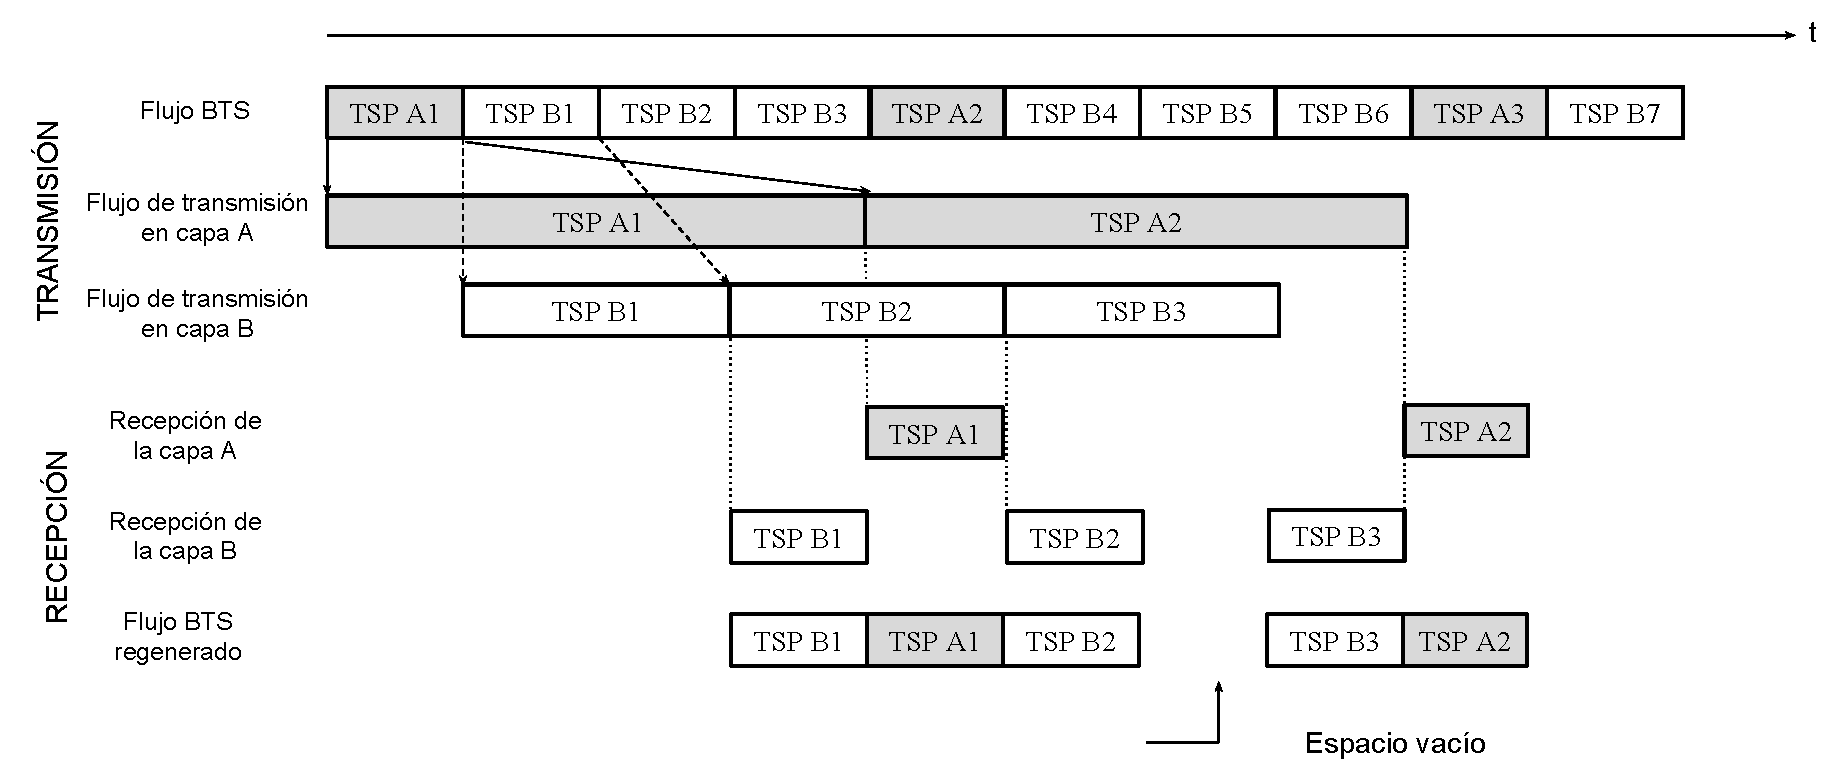
\includegraphics[width=3.5in]{figuras/bts1}
% where an .eps filename suffix will be assumed under latex, 
% and a .pdf suffix will be assumed for pdflatex; or what has been declared
% via \DeclareGraphicsExtensions.
\caption{Patrón de ordenamiento incorrecto del BTS.}
\label{bts1}
\end{figure}

\noindent pueda reconstruirlo perfectamente sin necesidad de la ISDB-T information. Supongamos que tenemos un BTS como el de la figura 2.4 en el cual hay dos capas jerárquicas A y B, cada una con su respectiva tasa tal que $r_{BTS} > r_B > r_A$. Las capas con tasas altas implican un tiempo de transmisión de paquetes mucho más corto que las capas con tasas bajas, y viceversa. Observando el diagrama de la figura \ref{bts1} puede verse que en recepción el paquete B1 es procesado antes de que termine de ser transmitido el paquete A1, cuando en realidad el orden original era A1 y luego B1. Además se generan espacios de tiempo en los cuales no se entregan paquetes al sistema porque aún se están procesando paquetes que van arribando. Esos intervalos de tiempo deben ser rellenados con paquetes nulos a fin de mantener la tasa constante. Esto resulta en un desordenamiento del patrón original del BTS y de la pérdida total de la capacidad de reordenar los datos en recepción.

Para formar los patrones de ordenamiento en transmisión de manera tal que
el receptor sea capaz de recuperarlos perfectamente, se agregan los denominados ajustes de atraso. En el ejemplo de la figura \ref{bts2} se agrega un ajuste de atraso de 2 TSP y se introduce un paquete nulo en el BTS original. Como resultado, el flujo BTS reconstruído por el receptor resulta ser exactamente igual al BTS original. Dada una configuración jerárquica del sistema, existe un único patrón de ordenamiento del BTS.

El transmisor implementado en este trabajo toma como flujo de entrada un
BTS ya conformado, y con la información jerárquica de los TSP es que logra
procesar cada capa por separado. De ahí en adelante las capas son entrelazadas y moduladas cada una de acuerdo a su propia configuración.

\begin{figure}[!h]
\centering
%\captionsetup{justification=centering}
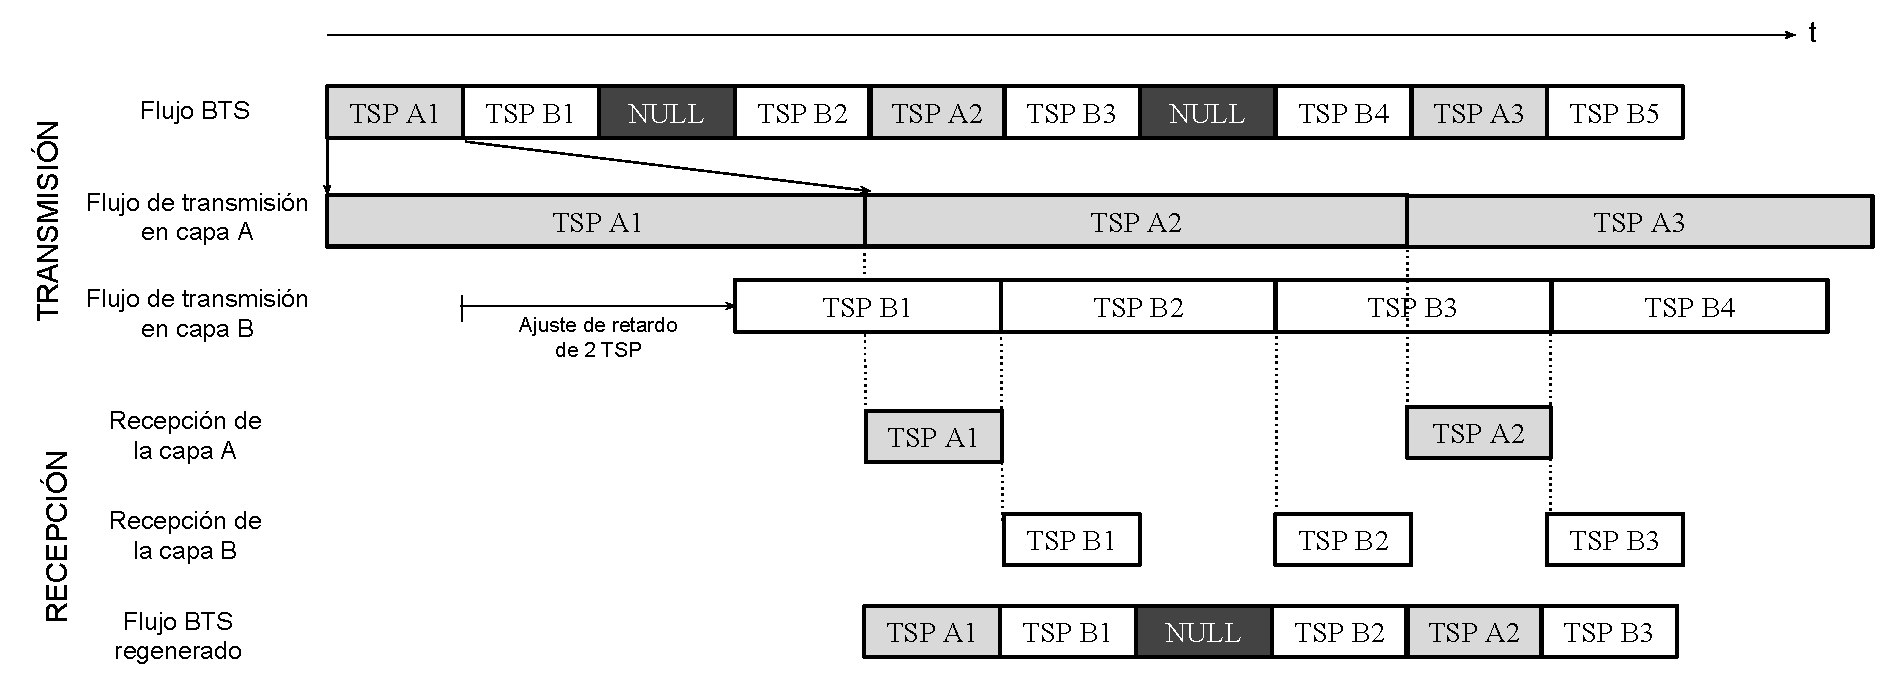
\includegraphics[width=3.5in]{figuras/bts2}
% where an .eps filename suffix will be assumed under latex, 
% and a .pdf suffix will be assumed for pdflatex; or what has been declared
% via \DeclareGraphicsExtensions.
\caption{Patrón de ordenamiento correcto del BTS.}
\label{bts2}
\end{figure}

\section{La estructura de cuadro OFDM}

\section{Los ajustes de atraso y el sincronismo}
Los bloques de entrelazamiento introducen atrasos. Estos atrasos son producto de los retardos variables a los que se someten los bytes, bits o símbolos complejos. Para que el sistema funcione correctamente el atraso total introducido por cada bloque debe ser un múltiplo de cuadro OFDM. Esto es un detalle importante que se tuvo en cuenta en el desarrollo de \textit{gr-isdbt-tx}, por lo que entendemos necesario desarrollar el concepto del ajuste de atraso.


\subsection{Ajuste de atraso en el entrelazamiento de byte}


\subsection{Ajuste de atraso en el entrelazamiento de bits}
En este entrelazamiento se utilizan 2, 4 ó 6 colas dependiendo si la modulación utilizada es QPSK, 16QAM, o 64QAM respectivamente. El tamaño de las colas, $q_i$, viene definido por el estándar. Por ejemplo para 64QAM los tamaños son $q_0 = 0$, $q_1 = 40$, $q_2 = 80$, $q_3 = 120$. Cualquiera sea la modulación el retardo máximo siempre es de 120 bits. Sin embargo vamos a dejarlo paramétrico en $q_i$ a fin de calcular el ajuste de atraso que es necesario introducir a cada cola.

El retardo agregado por el proceso corresponde al camino más largo que deben atravesar los bits, es decir un retardo de 120 símbolos. Según
la modulación que utilice la capa, estos 120 símbolos se traducen en un mayor o menor retardo en el tiempo; para QPSK corresponde a esperar que ingresen $120 \times 2$ bits en la entrada, mientras que para 64QAM deben pasar $120 \times 6$ bits.

Como los retardos deben ser siempre múltiplos de símbolos OFDM, el tamaño de un símbolo OFDM corresponde a:

\begin{equation}
N_{OFDM} = m_L \times N_L \times 96 \times 2^{modo - 1} \quad bits
\end{equation}

$N_{OFDM}$ depende de la cantidad de segmentos utilizados $N_L$, del modo de transmisión y de la modulación de la capa $m_L \in \{2,4,6\}$.

La solución implementada en este bloque es distinta a la del entrelazador de bytes. Aquí, el retardo total se obtiene incrementando los tamaños de las colas de manera que el retardo total sea de dos símbolos OFDM para cada capa. Por lo tanto para tener el retardo deseado los tamaños de las colas deben ser:

\begin{equation}
Q_i = q_i + \dfrac{2 \times N_{OFDM} -120 \times m_L}{m_L}
\end{equation}


\begin{equation}
Q_i = q_i +  N_L \times 96 \times 2^{modo - 1} - 120
\end{equation}

Una vez que son empujados los bits en cada cola, desde el otro extremo se extrae un bit por cola y se mapean en un símbolo complejo de acuerdo a lo establecido en la norma.

\subsection{Ajuste de atraso en el entrelazamiento temporal}
En el caso del entrelazamiento temporal, los símbolos complejos que arriban al bloque son encolados de manera secuencial en búfers de tamaño definido por la siguiente expresión:

\begin{equation}
q_L(i) = I_L \times ((i \times 5) \; mod \; 96)
\end{equation}

\noindent donde $i \in [0, 96 \times 2^{modo-1}]$ representa el número de portadora e $I_L$ es la profundidad del entrelazamiento y puede tomar los valores de la tabla \ref{parametros_ISDBT}.

Este proceso genera un atraso de $95 \times I_L \; mod \; 204$ símbolos, entonces para completar un cuadro OFDM hacen falta:

\begin{equation}
d_I = 204 - (95 \times I_L \; mod \; 204) 
\end{equation}

\noindent símbolos OFDM. Por lo tanto el retardo total en cuadros OFDM introducido por el proceso será:

\begin{equation}
N_L = (95 \times I_L + d_I) \; mod \; 204
\end{equation}

La implementación en el transmisor de este ajuste de atraso consiste en empujar los símbolos que arriban al bloque a cada una de las colas de tamaño $I_L \times (i \times 5) \; mod \; 96 + d_I$. Del otro extremo de las colas se toman los símbolos secuencialmente y se tiene la secuencia entrelazada. Este mecanismo, al igual que otros entrelazamientos, hace que en el arranque del sistema se tengan datos espurios en los registros.



\section{Pruebas}

\subsection{Subsection Heading Here}
Subsection text here.

% needed in second column of first page if using \IEEEpubid
%\IEEEpubidadjcol

\subsubsection{Subsubsection Heading Here}
Subsubsection text here.


% An example of a floating figure using the graphicx package.
% Note that \label must occur AFTER (or within) \caption.
% For figures, \caption should occur after the \includegraphics.
% Note that IEEEtran v1.7 and later has special internal code that
% is designed to preserve the operation of \label within \caption
% even when the captionsoff option is in effect. However, because
% of issues like this, it may be the safest practice to put all your
% \label just after \caption rather than within \caption{}.
%
% Reminder: the "draftcls" or "draftclsnofoot", not "draft", class
% option should be used if it is desired that the figures are to be
% displayed while in draft mode.
%
%\begin{figure}[!t]
%\centering
%\includegraphics[width=2.5in]{myfigure}
% where an .eps filename suffix will be assumed under latex, 
% and a .pdf suffix will be assumed for pdflatex; or what has been declared
% via \DeclareGraphicsExtensions.
%\caption{Simulation results for the network.}
%\label{fig_sim}
%\end{figure}

% Note that the IEEE typically puts floats only at the top, even when this
% results in a large percentage of a column being occupied by floats.


% An example of a double column floating figure using two subfigures.
% (The subfig.sty package must be loaded for this to work.)
% The subfigure \label commands are set within each subfloat command,
% and the \label for the overall figure must come after \caption.
% \hfil is used as a separator to get equal spacing.
% Watch out that the combined width of all the subfigures on a 
% line do not exceed the text width or a line break will occur.
%
%\begin{figure*}[!t]
%\centering
%\subfloat[Case I]{\includegraphics[width=2.5in]{box}%
%\label{fig_first_case}}
%\hfil
%\subfloat[Case II]{\includegraphics[width=2.5in]{box}%
%\label{fig_second_case}}
%\caption{Simulation results for the network.}
%\label{fig_sim}
%\end{figure*}
%
% Note that often IEEE papers with subfigures do not employ subfigure
% captions (using the optional argument to \subfloat[]), but instead will
% reference/describe all of them (a), (b), etc., within the main caption.
% Be aware that for subfig.sty to generate the (a), (b), etc., subfigure
% labels, the optional argument to \subfloat must be present. If a
% subcaption is not desired, just leave its contents blank,
% e.g., \subfloat[].


% An example of a floating table. Note that, for IEEE style tables, the
% \caption command should come BEFORE the table and, given that table
% captions serve much like titles, are usually capitalized except for words
% such as a, an, and, as, at, but, by, for, in, nor, of, on, or, the, to
% and up, which are usually not capitalized unless they are the first or
% last word of the caption. Table text will default to \footnotesize as
% the IEEE normally uses this smaller font for tables.
% The \label must come after \caption as always.
%
%\begin{table}[!t]
%% increase table row spacing, adjust to taste
%\renewcommand{\arraystretch}{1.3}
% if using array.sty, it might be a good idea to tweak the value of
% \extrarowheight as needed to properly center the text within the cells
%\caption{An Example of a Table}
%\label{table_example}
%\centering
%% Some packages, such as MDW tools, offer better commands for making tables
%% than the plain LaTeX2e tabular which is used here.
%\begin{tabular}{|c||c|}
%\hline
%One & Two\\
%\hline
%Three & Four\\
%\hline
%\end{tabular}
%\end{table}


% Note that the IEEE does not put floats in the very first column
% - or typically anywhere on the first page for that matter. Also,
% in-text middle ("here") positioning is typically not used, but it
% is allowed and encouraged for Computer Society conferences (but
% not Computer Society journals). Most IEEE journals/conferences use
% top floats exclusively. 
% Note that, LaTeX2e, unlike IEEE journals/conferences, places
% footnotes above bottom floats. This can be corrected via the
% \fnbelowfloat command of the stfloats package.




\section{Conclusiones}
The conclusion goes here.





% if have a single appendix:
%\appendix[Proof of the Zonklar Equations]
% or
%\appendix  % for no appendix heading
% do not use \section anymore after \appendix, only \section*
% is possibly needed

% use appendices with more than one appendix
% then use \section to start each appendix
% you must declare a \section before using any
% \subsection or using \label (\appendices by itself
% starts a section numbered zero.)
%


\appendices
\section{Proof of the First Zonklar Equation}
Appendix one text goes here.

% you can choose not to have a title for an appendix
% if you want by leaving the argument blank
\section{}
Appendix two text goes here.


% use section* for acknowledgment
\section*{Acknowledgment}


The authors would like to thank...


% Can use something like this to put references on a page
% by themselves when using endfloat and the captionsoff option.
\ifCLASSOPTIONcaptionsoff
  \newpage
\fi



% trigger a \newpage just before the given reference
% number - used to balance the columns on the last page
% adjust value as needed - may need to be readjusted if
% the document is modified later
%\IEEEtriggeratref{8}
% The "triggered" command can be changed if desired:
%\IEEEtriggercmd{\enlargethispage{-5in}}

% references section

% can use a bibliography generated by BibTeX as a .bbl file
% BibTeX documentation can be easily obtained at:
% http://mirror.ctan.org/biblio/bibtex/contrib/doc/
% The IEEEtran BibTeX style support page is at:
% http://www.michaelshell.org/tex/ieeetran/bibtex/
%\bibliographystyle{IEEEtran}
% argument is your BibTeX string definitions and bibliography database(s)
%\bibliography{IEEEabrv,../bib/paper}
%
% <OR> manually copy in the resultant .bbl file
% set second argument of \begin to the number of references
% (used to reserve space for the reference number labels box)
%\begin{thebibliography}{1}
%
%\bibitem{IEEEhowto:kopka}
%H.~Kopka and P.~W. Daly, \emph{A Guide to \LaTeX}, 3rd~ed.\hskip 1em plus
%  0.5em minus 0.4em\relax Harlow, England: Addison-Wesley, 1999.
%
%\bibitem{gr-isdbt-tx}
%Javier~Hernández, Santiago~Castro, \emph{gr-isdbt-tx}. [Online]. Disponible: \relax https://github.com/jhernandezbaraibar/gr-isdbt-Tx
%
%\bibitem{norma}
%ARIB, "Transmission System for Digital Terrestrial Television Broadcasting". 2014. [Online]. Disponible: https://www.arib.or.jp/english/html/overview/doc/6-STD-B31v1\_6-E2.pdf
%
%\bibitem{winCom16}
%Federico Larroca, Pablo Flores-Guridi, "An open and free {ISDB-T} full seg receiver implemented in GNU Radio". 2016. [Online]. Disponible: https://iie.fing.edu.uy/publicaciones/2016/LFGGB16/LFGGB16.pdf
%
%
%
%
%
%
%\bibitem{chang-ofdm,
%  title={Synthesis of band-limited orthogonal signals for multichannel data transmission},
%  author={Chang, Robert W},
%  journal={Bell System Technical Journal},
%  volume={45},
%  number={10},
%  pages={1775--1796},
%  year={1966},
%  publisher={Wiley Online Library}
%}
%
%\end{thebibliography}\\\

\bibliographystyle{IEEEtran}
\bibliography{IEEEabrv}

% biography section
% 
% If you have an EPS/PDF photo (graphicx package needed) extra braces are
% needed around the contents of the optional argument to biography to prevent
% the LaTeX parser from getting confused when it sees the complicated
% \includegraphics command within an optional argument. (You could create
% your own custom macro containing the \includegraphics command to make things
% simpler here.)
%\begin{IEEEbiography}[{\includegraphics[width=1in,height=1.25in,clip,keepaspectratio]{mshell}}]{Michael Shell}
% or if you just want to reserve a space for a photo:

% insert where needed to balance the two columns on the last page with
% biographies
%\newpage


% You can push biographies down or up by placing
% a \vfill before or after them. The appropriate
% use of \vfill depends on what kind of text is
% on the last page and whether or not the columns
% are being equalized.

%\vfill

% Can be used to pull up biographies so that the bottom of the last one
% is flush with the other column.
%\enlargethispage{-5in}



% that's all folks
\end{document}


